% !TeX encoding = UTF-8
% !TeX program = pdflatex
% !TeX spellcheck = it_IT

%Pubblico il seguente file per condividere con i miei compagni di corso la struttura da me configurata per la tesi in medicina e chirurgia al Sant'Andrea  

%Qui tutto ciò che c’ è da saper su LaTeX: http://www.lorenzopantieri.net/LaTeX_files/ArteLaTeX.pdf 
%Per scrivere la bibliografia puoi vedere il seguente link: https://www.guitex.org/home/images/doc/GuideGuIT/bibliografia.pdf

\documentclass[a4paper, oneside]{sapthesis}

%qui ci sono svariati pacchetti utili per far funzionare il programma
\usepackage{microtype}
\usepackage[italian]{babel}
\usepackage[utf8]{inputenc}
\usepackage{imakeidx}
\usepackage{subfigure}
\usepackage[acronym]{glossaries}
\usepackage{graphicx}
\captionsetup{labelsep=quad}
\usepackage{array}
\usepackage{ragged2e}
\usepackage[table]{xcolor}
\usepackage{hyperref}
\usepackage{blindtext}


% Miei include
\usepackage{amsfonts} 
\usepackage{amsmath}

\usepackage{pgfplots}
\pgfplotsset{compat=1.18}

\usepackage{svg}

\usepackage[linguistics]{forest} %per dare i diagrammi: https://texdoc.org/serve/forest/0

\newcommand*{\belowrulesepcolor}[1]{% 
  \noalign{% 
  \kern-\belowrulesep \begingroup \color{#1}% 
  \hrule height\belowrulesep \endgroup }%
}
\newcommand*{\aboverulesepcolor}[1]{% 
  \noalign{%
  \begingroup \color{#1}% 
  \hrule height\aboverulesep \endgroup \kern-\aboverulesep }%
}

\usepackage[sort]{natbib}
\bibliographystyle{plainyr-rev} %la bibiografia ordinata in ordine di data dalla più recente
\setcitestyle{super,open={(},close={)}}

\hypersetup{pdftitle={TITOLO TESI}, pdfauthor={Luca Sforza}}
\title{Simulazione di Modelli Biologici riguardanti varie forme del carcinoma}
\author{Luca Sforza}
\IDnumber{2050030}
\course{Laurea triennale in Informatica}
\courseorganizer{Facoltà di Ingegneria dell'informazione, informatica e statistica} % TODO: controllare
\AcademicYear{2024/2025}
\advisor{Dott. Enrico Tronci}
\customadvisorlabel{Relatore}
%\coadvisor{Dott.ssa Nome Cognome}
%\customcoadvisorlabel{Correlatrice}
%\director{Dott.  Nome Cognome}
%\customdirectorlabel{Specializzando\\Responsabile della ricerca}
\authoremail{sforza.2050030@studenti.uniroma1.it}
\copyyear{2025}
\thesistype{Tesi sperimentale}
\examdate{24 Gennaio 2024} % TODO: boh
\examiner{Prof. Tizio} 
\examiner{Prof. Caio} 
\examiner{Prof. Sempronio}  
\examiner{Prof. ...}  
\examiner{Prof. ...} 
\examiner{Prof. ...}  
\examiner{Prof. ...} 

%In caso di titoli di section a 2 righe
%\setlength{\headheight}{22.59052pt}
%\addtolength{\topmargin}{-10.59052pt}

\makeindex
\makeglossaries
\newglossaryentry{PROVA}
{
        name=NOME DELLA VOCE GLOSSARIO,
        description={DESCRIZIONE DELLA VOCE GLOSSARIO}
}

\newacronym{GLOSSARIO}{GLOSSARIO}{\gls{PROVA}}


\includeonly{Cap_1,Cap_2,Cap_3,Cap_4,Cap_5}
\newcommand{\Fig}[1]{[{\footnotesize \texttt{Fig.#1}}]}
\newcommand{\citfig}[1]{\ap{\scriptsize\textrm{(\textit{F#1})}}}

\begin{document}
\frontmatter
\maketitle
\dedication{
\begin{flushright}
\emph{«Tutti i modelli sono sbagliati, ma alcuni sono utili.»}\\
--- George E. P. Box
\end{flushright}
}

\begin{abstract}

\paragraph{Contesto}


\paragraph{Obbiettivi}


\paragraph{Metodi} 

\paragraph{Risultati}

\paragraph{Conclusione}

\end{abstract}
\tableofcontents
\listoffigures
\listoftables

\phantomsection
\addcontentsline{toc}{chapter}{Acronomi}
\printglossary[type=\acronymtype]

\mainmatter
\chapter{Introduzione}
Ciao \citep{guit}
\chapter{Modellazione Biologica}

\section{Introduzione}

I modelli biologici che consideriamo sono sistemi dinamici tempo-invarianti, generalmente non lineari, descritti da equazioni differenziali ordinarie (ODE).

Lo stato del sistema al tempo \(t\) è un vettore \(x(t) = (x_1(t),\dots,x_n(t))^\top \in [0,1]^n \subseteq \mathbb{R}^n\), dove \(x_i(t)\) rappresenta la concentrazione normalizzata della i-esima specie. Poiché le concentrazioni sono normalizzate, \(x_i(t)\in[0,1]\) per ogni \(i\) e ogni \(t\).

In forma compatta le ODE si scrivono
\[
\frac{dx}{dt} = f(t,x).
\]

Sia \(m\) il numero di reazioni nel modello.

Per ogni specie \(x_i\) definiamo
$R_{x_i} \subseteq \{1,\dots,m\}\quad\text{(reazioni in cui \(x_i\) è reattante)}$,
$P_{x_i} \subseteq \{1,\dots,m\}\quad\text{(reazioni che producono \(x_i\))}.$

Se \(R_{x_i}\neq\emptyset\) e \(P_{x_i}\neq\emptyset\), l'evoluzione temporale di \(x_i\) è data da:
\[
\frac{dx_i}{dt}=\sum_{j\in P_{x_i}} v_j(t) - \sum_{j\in R_{x_i}} v_j(t),
\]
dove \(v_j(t)\) è la velocità della reazione \(j\).

La velocità di una reazione è data dalla legge dell'azione di massa (mass action).

La velocità di una reazione chimica è proporzionale al prodotto delle concentrazioni dei reagenti, ciascuna elevata al proprio coefficiente stechiometrico

La velocità di una reazione è influenzata da modificatori (enzimi, inibitori). Per modellare l'effetto dei modificatori si usa spesso la funzione di Hill. Per ogni specie modificatrice \(x_\ell\) introduciamo una funzione di Hill generica
\[
H_\ell(t) =
\begin{cases}
\dfrac{x_\ell(t)^{10}}{K_\ell + x_\ell(t)^{10}}, &\text{se \(x_\ell\) agisce da attivatore},\\[8pt]
\dfrac{K_\ell}{K_\ell + x_\ell(t)^{10}}, &\text{se \(x_\ell\) agisce da inibitore},
\end{cases}
\]
dove \(K_\ell>0\) è la costante di mezzo-saturazione e dato che è ingnota viene aggiunta cime parametro del modello.

Per la reazione \(i\in\{1,\dots,m\}\) definiamo inoltre:


$S_i=\{j\in\{1,\dots,n\}\mid x_j \text{ è reattante della reazione } i\}$,


$M_i=\{j\in\{1,\dots,n\}\mid x_j \text{ è modificatore della reazione } i\}$.

$n_i^j$ è la stochiometria della specie $j$ nella reazione $i$.

La velocità \(v_i(t)\) si esprime quindi come
\[
v_i(t)=k_i\;\prod_{j\in S_i} x_j(t)^{n_i^j}\;\prod_{j\in M_i} H_j(t),
\]
dove \(k_i>0\) è la costante cinetica della reazione. Essa essendo sconosciuta viene aggiunta
come parametri del modello.

\section{modelli biologici di Pathway}

Un pathway metabolico (o via metabolica)  è una sequenza di reazioni biochimiche che collega metaboliti chiave.

Un pathway è formato da specie di input che non vengono prodotte da reazioni, ma vengono immesse nel pathway.
Specie intermedie che sono sia prodotte che consumate da reazioni, specie di output che sono solo prodotte da reazioni e mai consumate
e specie che non vengono ne prodotte ne consumate da alcuna reazione, ma sono enzimi o inibitori che influscono nelle altre reazioni.

Un esempio tipico di input è l'ATP che funge da "energia" per molte reazioni chimiche.

Esse non vengono prodotte da reazioni (\(P_{x_i}=\emptyset\)) ma vengono immesse nel sistema; si modellano con un termine di ingresso constante \(k_{\mathrm{in},i}\):

\[
\frac{dx_i}{dt}=k_{\mathrm{in},i} - \sum_{j\in R_{x_i}} v_j(t).
\]

I pathway hanno degli output che sono specie che vengono prodotte ma non consumate (\(R_{x_i}=\emptyset\)); ad esse si aggiunge una reazione di degradazione, che avrà una constante cinetica e ha come unico reattante
la concentrazione dell'output stesso, quindi seguendo la mass action rule l'equazione differenziale per gli output è come segue:
\[
\frac{dx_i}{dt}=\sum_{j\in P_{x_i}} v_j(t) - k_{\mathrm{out},i}\,x_i(t),
\]

Nei modelli biologici di pathway possono essere presenti specie che non partecipano ne come reattanti ne come prodotti alle reazioni, ma solo come
modificatori. Quindi queste specie devono avere una costante di immissione ed anche una di degradazione.

Queste specie sono enzimi o inibitori esterni, quindi influiscono sulla velocità delle altre reazioni del modello. La loro dinamica è descritta come segue:
\[
\frac{dx_i}{dt}=k_{\mathrm{in},i}-k_{\mathrm{out},i}\,x_i(t).
\]


\chapter{Stima dei parametri}

Le costanti cinetiche e gli altri parametri (es. \(K_\ell\), \(k_{\mathrm{in},i}\), \(k_{\mathrm{out},i}\)) sono generalmente sconosciuti e devono essere stimati. 
Poiché i parametri cinetici possono variare di molti ordini di grandezza, è comune parametrizzarli in scala logaritmica. 
Se \(p\) è il numero totale di parametri, si può usare un vettore di parametri \(\theta\in [-20,20]^p \subseteq \mathbb{Z}^p\).

Da notare che il dominio dei parametri è non solo discreto, ma addirittura finito. Questo ci permetterà di cercare tutti i parametri che rispettono determinati vincoli.

Per ricavare la costante cinetica a partire dal parametro logaritmico si usa la parametrizzazione in base dieci:
\[
k_i = 10^{\theta_i}, \qquad \theta_i \in [-20,20],
\]
così \(\theta_i\) rappresenta \(\log_{10} k_i\) e si garantisce \(k_i>0\).


Prima di stimare i parametri bisogna aggiungere dei vincoli su di essi.

Si può fare in due modi: o limitando il dominio delle constanti cinetiche eliminando quelle implausibili oppure
definendo una funzione che dati i parametri valutano l'errore all'interno del modello, poi tramite un ottimizzatore black box si trovano 
i parametri che minimizzano l'errore.

Per l'esame di \textbf{intelligenza artificiale} su cui si basa il progetto del tirocinio è stato mostrato
quale algoritmo dell'ottimizzatore Nevergrad converge più velocemente su un modello particolare e semplificato.

\section{Vincoli sui parametri}

I parametri da scegliere devono soddisfare determinati requisitivi.

Primo tra tutti i parametri devono rendenre il sistema stabile.

Quindi bisogna notare il fatto che gli enzimi o inibitori di una reazione controllano il comportamento di quella reazione.

Quindi una condizione necessaria, ma non sufficiente per la stabilità è che le constanti cinetiche che producono modificatori (enzimi o inibitori)
devono essere maggiori delle constanti cinetiche che i modificatori alterano.

Formalmente sia: 
\[
    R = \{(i,j) \in [1,m]^2 \mid \text{ la reazione } i \text{ produce un modificatore della reazione } j\}
\]

Allora l'ottimizzatore deve rispettare questi vincoli che limitano lo spazio feaseble dei parametri:

\begin{equation}
    k_i \geq  k_j \mid (i,j) \in R
\end{equation}

Per vincolare defenitivamente la stabilità bisogna eliminare il transitorio. Il transitorio è la parte
iniziale del sistema in cui i valori non sono ancora stabili.

Per capire cos'è il transitorio dobbiamo definire cos'è la concentrazione media di una specie.

Definiamo $T$ come l'orizzonte di simulazione.

La concentrazione di una specie non dipende solo dal tempo, ma anche dai parametri, quindi la concentrazione di una specie è: $x_i(t,\theta)$.

La concentrazione media di una specie $i$ è definita come segue:

\begin{equation}
    \tilde{x}_i(t',\theta)
    = \mathbb{E}_{\tau\sim\mathcal{U}(0,t')} \big[ x_i(\tau,\theta) \big]
    = \frac{1}{t'} \int_{0}^{t'} x_i(\tau,\theta)\,d\tau,\qquad t'>0.
\end{equation}

\begin{figure}
\centering
    
\begin{tikzpicture}
\begin{axis}[
    xlabel={Tempo $t$},
    ylabel={Concentrazione $x_i(t)$},
    axis lines=left,
    width=10cm,
    height=6cm,
    grid=major,
    ymin=0,
    ymax=1,
]

% Esempio di andamento della concentrazione (blu)
\addplot[blue, thick, domain=0:10, samples=200] {0.4*(1 + sin(deg(2*pi*x/10))) + 0.1};

% Definizione dei punti medi
\def\T{10}
\def\xmedA{0.8}   % valore medio fino a T/2
\def\xmedB{0.4}   % valore medio fino a T

% Punti blu per le medie
\addplot[only marks, mark=*,
         mark options={fill=blue}, blue] coordinates {(5, \xmedA)};
\addplot[only marks, mark=*,
         mark options={fill=blue}, blue] coordinates {(10, \xmedB)};

% Segmento rosso (transitorio)
\addplot[green, thick] coordinates {(5, \xmedA) (0, \xmedA)};

\addplot[green, thick] coordinates {(10, \xmedB) (0, \xmedB)};

\addplot[red, thick] coordinates {(5, \xmedA) (5, \xmedB)};

% Etichette
\node[blue, above] at (axis cs:5,\xmedA) {$\tilde{x}_i(\phi \cdot T,\theta)$};
\node[blue, above] at (axis cs:9,\xmedB) {$\tilde{x}_i(T,\theta)$};
\node[text=red, above] at (axis cs:6.2,0.55) {Transitorio};
\end{axis}
\end{tikzpicture}
\caption{Visulizzazione del transitorio}
\label{fig:transitorio}
\end{figure}


Il transitorio quindi è il segmento tra i due valori medi \(\tilde{x}_i(\phi \cdot T,\theta)\) e \(\tilde{x}_i(T,\theta)\).

$\phi$ è un iper-parametro dell'ottimizzatore, per lo scopo del tirocinio è stato scelto $\phi = \frac{1}{2}$.

Per vincolare l'eliminazione del transitorio definiamo una funzione da minimizzare:

\begin{equation}
    \mathcal{L}_1(\theta) = \sum_{i=1}^n (\tilde{x}_i(\phi \cdot T, \theta) - \tilde{x}_i(T, \theta))^2
\end{equation}

Minimizzare $\mathcal{L}_1$ significa eliminare il transitorio e quindi vincolare la stabilità del sistema.

Per poter visulizzazione che cos'è il transitorio in figura \ref{fig:transitorio} è presente un esempio.

Un altro vincolo sulle constanti cinetiche è che devono far rimanere
il valore delle concentrazioni tra 0 e 1, poiché per ipotesi la concentrazioni delle specie sono tutte normalizate.

Per fare ciò dobbiamo aggiungere delle nuovi variabili allo stato per ogni specie esistente, con la relativa equazione differenziale:

$z_i$ è la nuova variabile dello stato associato alla specie $x_i$.

\begin{equation}
    \frac{d z_i}{d t} = \text{\textbf{if} } x_i(t, \theta) \geq 1 \lor x_i(t,\theta) \leq 0 \text{ \textbf{then} } 10 \text{ \textbf{else} } 0
\end{equation}

Quindi per vincolare le specie tra 0 e 1 dobbiamo minimizzare il valore di queste variabili.

\begin{equation}
    \mathcal{L}_2(\theta) = \sum_{i=1}^n z_i(T, \theta)
\end{equation}

I parametri delle constanti cinetiche non solo devono garantire la stabilità, ma devono anche
garantire varie regole biologiche. Per esempio l'acqua è il solvente della vita, tutto ciò che
è presente dentro una cellula è immerso nell'acqua. L'acqua quindi è sempre la specie più espressa all'interno di un modello biologico.

L'acqua è solo un esempio, ma esistono molti motivi del perché si vuole vincolare che una certa specie è più espressa di un altra.

Definiamo quindi una relazione di ordinamento sulle specie $R \subseteq [1,n]^2$.

Se $(i,j) \in R$ allora la specie $j$ deve essere più espressa della specie $i$.

Definiamo una nuove funzione da minimizzare $\mathcal{L}_3$.

\begin{equation}
    \mathcal{L}_3(\theta) = \sum_{(i,j) \in R} max(0, \tilde{x}_i(T, \theta) - \tilde{x}_j(T, \theta))
\end{equation}

Altri vincoli da aggiungere sono vincolare il valore medio di una concentrazione ad una certa constante nota.

Supponiamo di avere un dataset:
\[
    \mathcal{D} = \{ y_i \in [0,1] \mid y_i \text{ è la concentrazione media osservata della specie i}\}.
\]

Un modo per vincolare i parametri a questi dati è massimizzando la \textbf{likehood} dei parametri.

La likehood è la probabilità condizionata di osservate dal modello
il dato osservato se il modello è corretto.

Più formalmente:

\begin{equation}
    L(\theta \mid \mathcal{D}) = \mathbb{P}(\mathcal{D} \mid \theta)
\end{equation}

Quindi i parametri da scegliere devono essere quelli che massimizzano la likehood.

\begin{equation}
    \hat{\theta}(\mathcal{D}) = \arg\max_{\theta} L(\theta \mid \mathcal{D})
\end{equation}

Ma in pratica per ottenere questi parametri dobbiamo fare delle ipotesi.

I dati osservati $\mathcal{D}$ per ipotesi devono provenire da repliche sperimentali indipendenti ottenute nelle stesse condizioni sperimentali del modello e affette da rumore osservazionale. Tipicamente si assume un errore additivo gaussiano sulle medie osservate:
\[
y_i = \tilde{x}_i(T,\theta) + \varepsilon_i,\qquad \varepsilon_i \sim \mathcal{N}(0,\sigma_i^2),
\]
dove \(\sigma_i^2\) è la varianza dell'errore per la specie \(i\). Sotto questa ipotesi la log-likehood del dataset è
\[
\log L(\theta\mid\mathcal{D}) = -\frac{1}{2}\sum_{ y_i\in\mathcal{D}}\left[\frac{(y-\tilde{x}_i(T,\theta))^2}{\sigma_i^2} + \log(2\pi\sigma_i^2)\right].
\]
La stima dei parametri si ottiene massimizzando questa funzione (o minimizzando la somma dei residui normalizzati).

Quindi definiamo una nuova funziona da minimizzare $\mathcal{L}_4$.

\begin{equation}
    \mathcal{L}_4(\theta) = \sum_{y_i \in \mathcal{D}} (y_i - \tilde{x}_i(T,\theta))^2
\end{equation}

Come ultima funzione da definire è una per gestire gli errori numerici. Se la scelta delle costanti cinetiche è troppo sbagliata le specie potrebbero molto velocemente divergere a $+\infty$.

Perciò definiamo una funzione che da $+\infty$ nel caso la simulazione è terminata con errori numerici e 0 altrimenti.

\begin{equation}
    \mathcal{L}_5(\theta) = \begin{cases}
        +\infty \text{ se la simulazione è terminata con errori numerici}\\
        0 \text{ altrimenti}
    \end{cases}
\end{equation}

La funzione finale da minimizzare è:

\begin{equation}
    \mathcal{L}(\theta) = \alpha \cdot \mathcal{L}_1(\theta) + \beta \cdot \mathcal{L}_2(\theta) + \gamma \cdot \mathcal{L}_3(\theta) + \zeta \cdot \mathcal{L}_4(\theta) + \mathcal{L}_5(\theta)
\end{equation}

Dove $\alpha, \beta , \gamma, \zeta \in \mathbb{R}$ sono degli iperparametri dell'ottimizzatore per scalare
le varie funzioni a seconda se vogliamo vincolare di più l'aderenza ai dati sperimentali ($\gamma$ o $\zeta$) oppure la stabilità.

\section{Come trovare i parametri}

Per trovare i parametri è equivalente a dire che:

\begin{equation}
    \mathcal{S} = \arg\max_{\theta} \mathcal{L}(\theta)
\end{equation}

Dato che il dominio dei parametri è discrito potremmo poter trovare tutti i possibili parametri che rispettano i vincoli, ovvero tale per cui 
$\mathcal{L}(\theta) <= \epsilon$ dove $\epsilon > 0$ molto piccolo.

Se i parametri da cercare sono molto pochi allora si può provare a cercare tutte le soluzioni possibili.

Altrimenti si può utilizzare il risultato ottenuto dal progetto di \textbf{intelligenza artificiale} per trovare
tramite ottimizzazione black box i parametri migliori, anche se la differenza è che qua operiamo nel discreto e non con parametri continui.




\chapter{Esempi di modelli}


\begin{figure}[htbp]
    \centering
    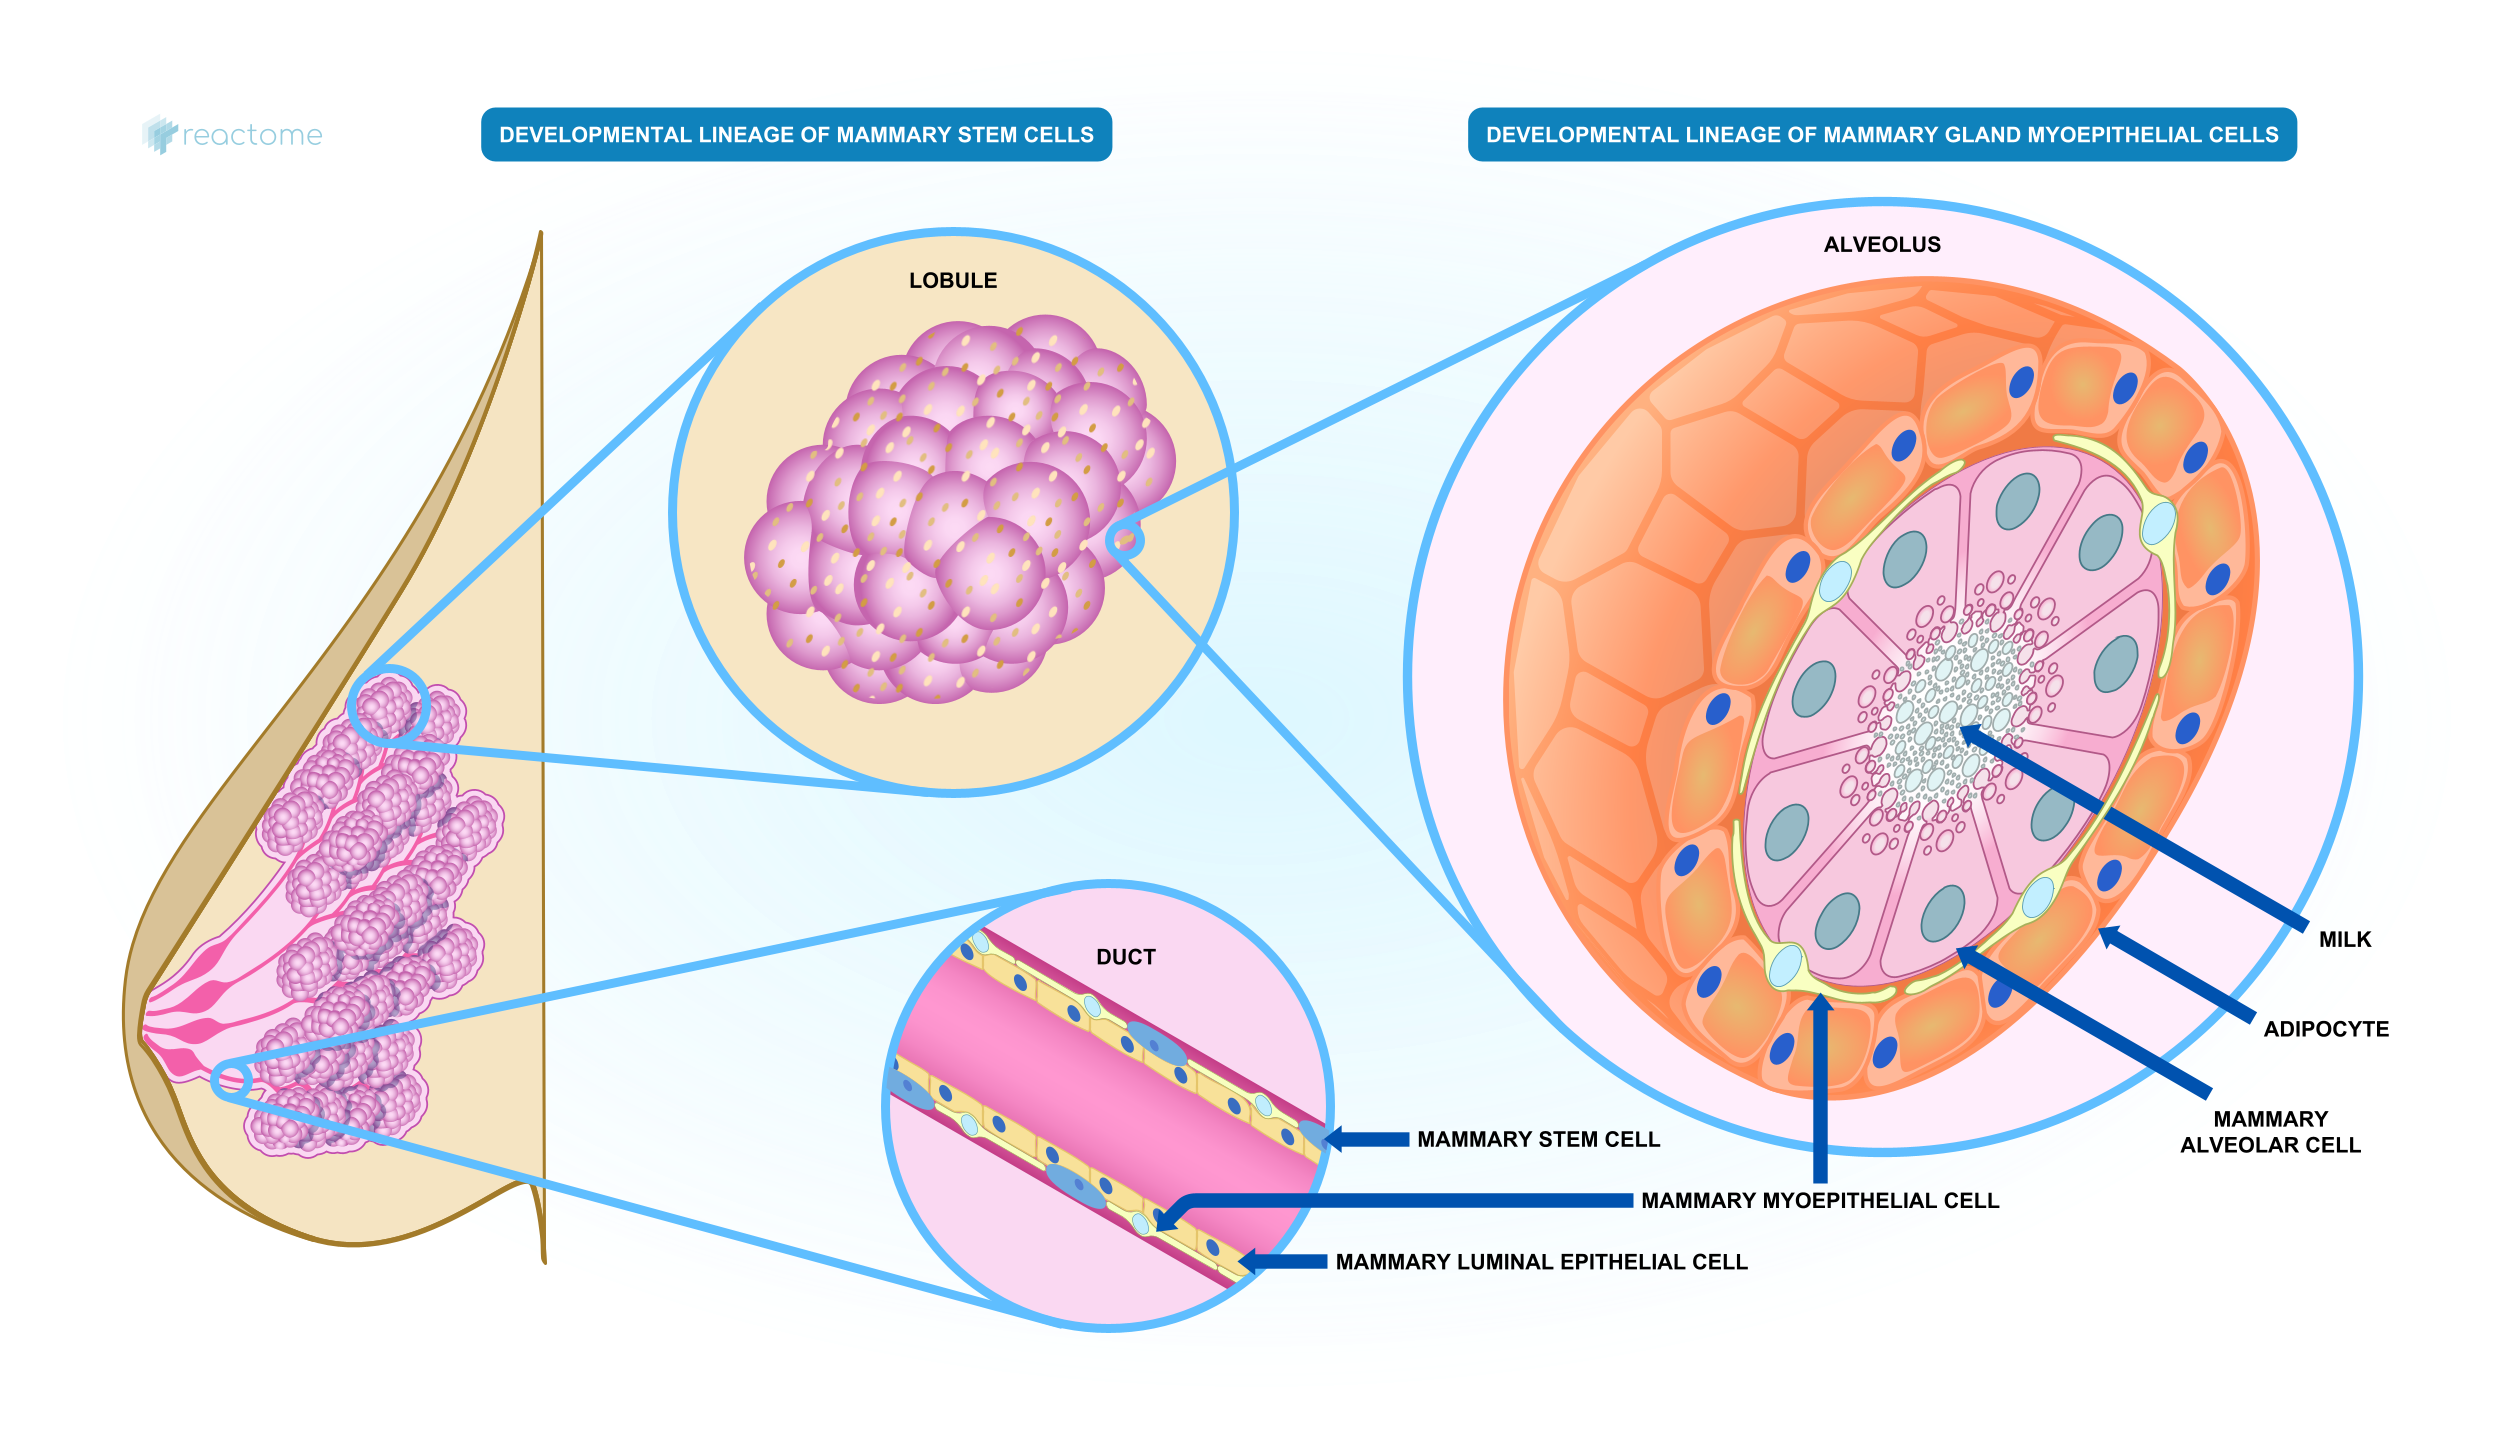
\includegraphics[width=\textwidth]{R-HSA-9938206.png}
    \caption{Rappresentazione del modello: R-HSA-9938206}
    \label{fig:R-HSA-9938206}
\end{figure}

Questo modello rappresenta lo sviluppo delle cellule staminali mammarie.

\begin{figure}[htbp]
    \centering
    \makebox[\textwidth][c]{%
        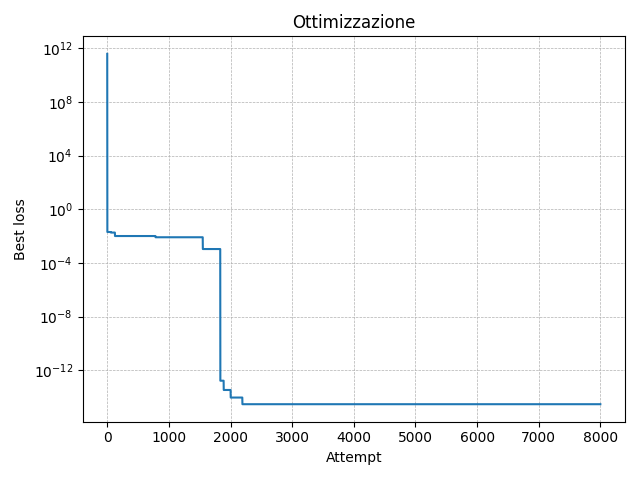
\includegraphics[width=0.5\textwidth]{plot_9938206.png}%
        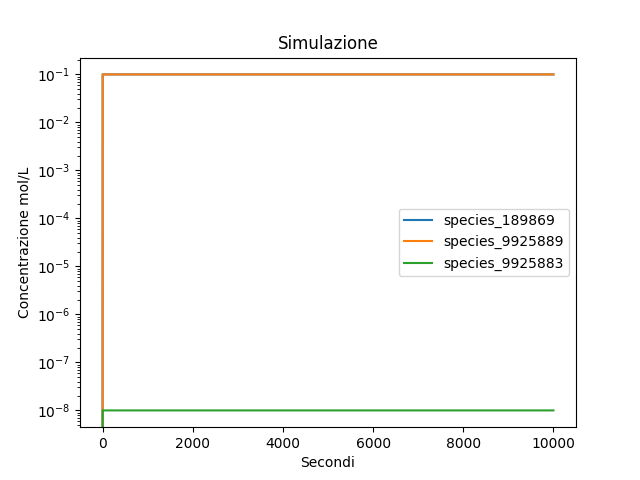
\includegraphics[width=0.5\textwidth]{simulation_9938206.png}%
    }%
    \caption{A sinistra c'è l'ottimizzazione fatta da Nevergrad dei parametri e a destra invece la simulazione.}
    \label{fig:due-immagini-affiancate}
\end{figure}

Il problema è stato vincolato in modo tale che le specie con id 189869 e 9925889 avessero come concentrazione media $0.1$ e che la specie 9925883 fosse la meno espressa.

Si possono vedere i risultati in \ref{fig:due-immagini-affiancate}

\begin{figure}[htbp]
    \centering
    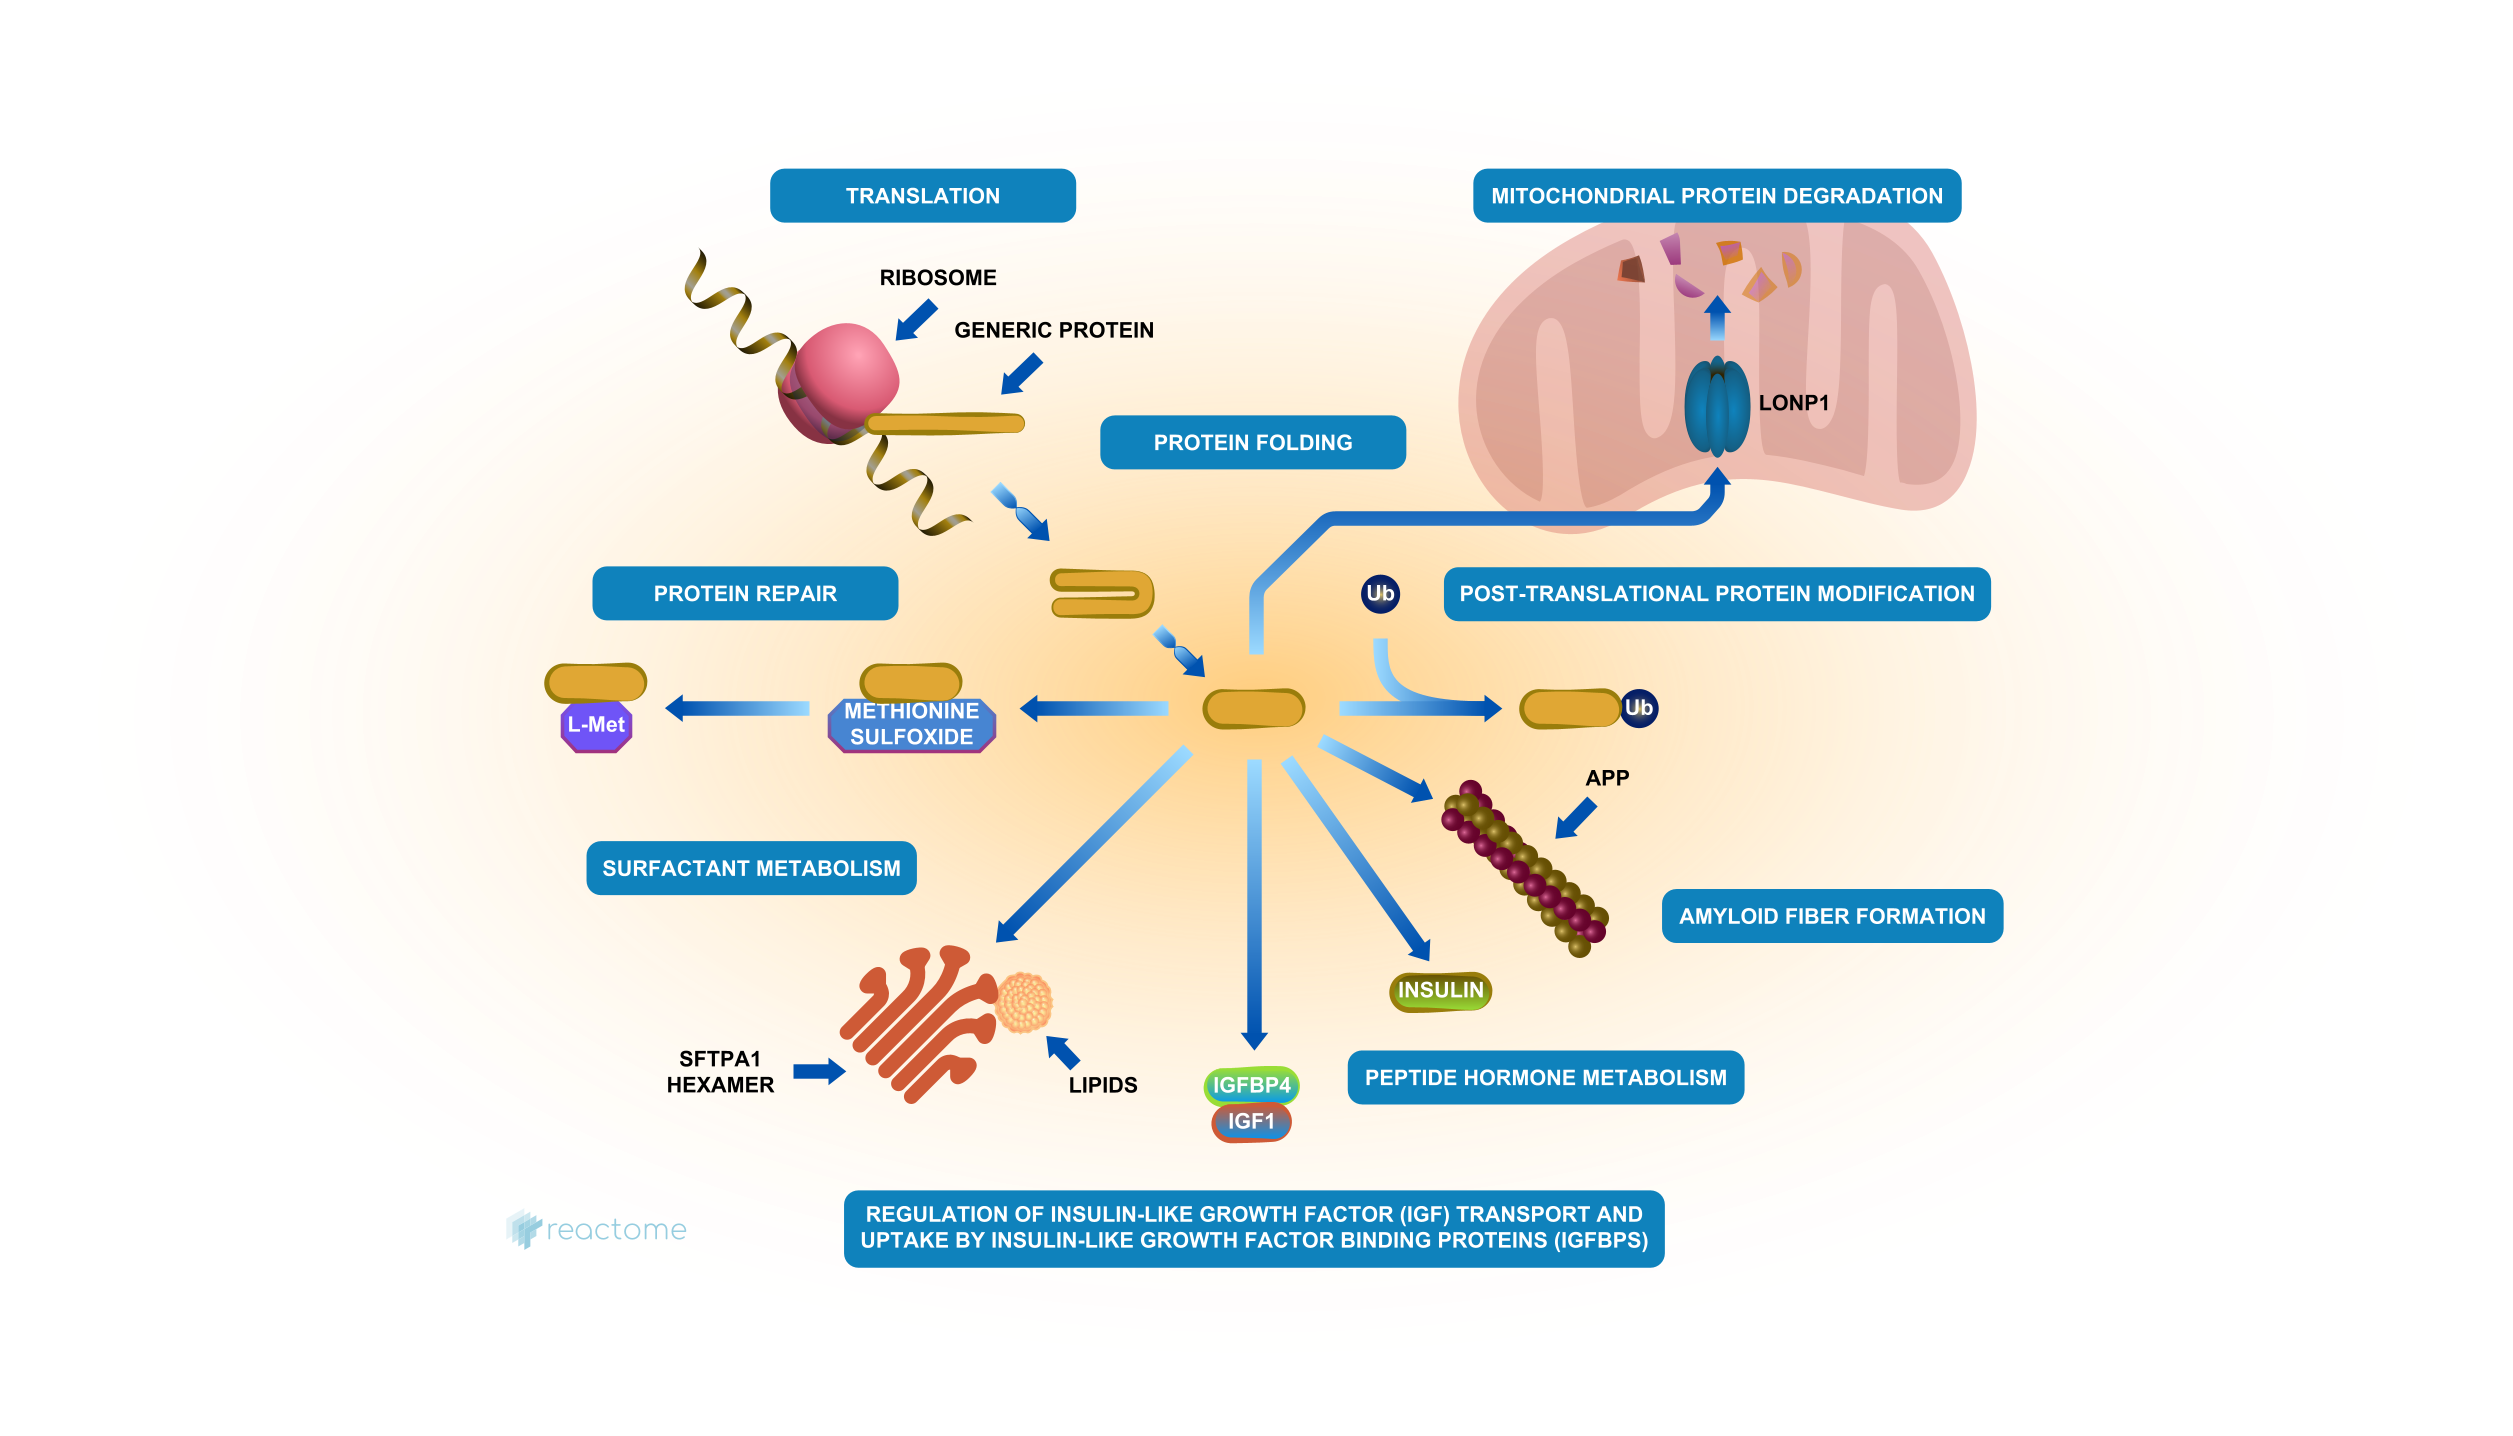
\includegraphics[width=\textwidth]{R-HSA-390471.png}
    \caption{Rappresentazione del modello: R-HSA-390471}
    \label{fig:R-HSA-390471}
\end{figure}

Per il modello \ref{fig:R-HSA-390471} è stata vincolata solo la stabilià e si possono vedere i risultati in \ref{fig:due-immagini-affiancate2}.

\begin{figure}[htbp]
    \centering
    \makebox[\textwidth][c]{%
        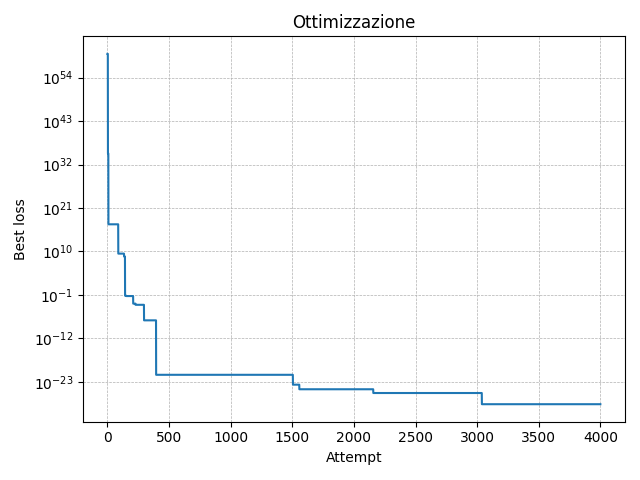
\includegraphics[width=0.5\textwidth]{plot_390471.png}%
        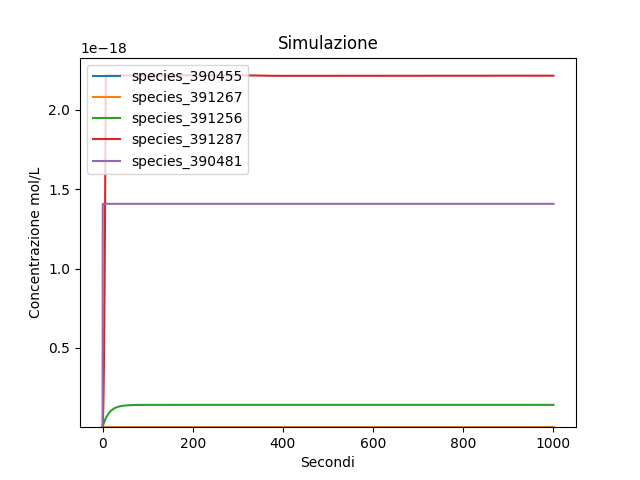
\includegraphics[width=0.5\textwidth]{simulation_390471.png}%
    }%
    \caption{A sinistra c'è l'ottimizzazione fatta da Nevergrad dei parametri e a destra invece la simulazione.}
    \label{fig:due-immagini-affiancate2}
\end{figure}
\chapter{Conclusione}
\section{Innovatività della ricerca}
\section{Potenzialità di realizzare un avanzamento delle conoscenze}

\backmatter
\cleardoublepage

\newpage
\phantomsection
\addcontentsline{toc}{chapter}{\glossaryname}
\printglossary

%\newpage
%\phantomsection
%\addcontentsline{toc}{chapter}{\indexname}
%\printindex

\newpage
\phantomsection
\addcontentsline{toc}{chapter}{\bibname}
\bibliography{bibiografia}

\newpage
\phantomsection
\addcontentsline{toc}{section}{Figure}

%\begin{acknowledgments}
\chapter{Ringraziamenti}

% Ringrazio dal profondo del cuore i miei genitori, per il loro affetto, la pazienza e il costante sostegno che mi hanno accompagnato lungo tutto il percorso accademico.

% Ringrazio anche Intesa San Paolo per avermi messo una spada di damocle sulla testa che mi ha costretto a dare tutti gli esami in tempo.

% Desidero esprimere la mia gratitudine al mio relatore per la preziosa guida, la disponibilità e i continui stimoli intellettuali che hanno reso possibile questo lavoro.

% TODO: da completare



%\end{acknowledgments}

\end{document}